\section{Integration in CLAS12}
\label{sec:integration}

The FT mechanical design was driven by the geometrical constraints imposed by the other CLAS12 sub-detectors,
geometrical acceptance optimization, and performance optimization, taking into account cooling, material budget, and
front-end electronics location. The FT detects electrons scattered between $2.5^\circ$ and $4.5^\circ$ with respect
to the beam axis. To provide this acceptance, the FT calorimeter must cover down to $2^\circ$ and up to $5^\circ$ with
lead tungstate crystals to have a good containment of electromagnetic showers at the edges of the polar angular range.
Since no massive materials are allowed at angles larger than $5.5^\circ$, the crystals, cooling system, mechanical
supports, and tungsten shielding have been optimized in a very compact design. Outside of $5.5^\circ$ the only
materials are very low-density (35~kg/m$^3$) insulation and routing for cabling and services in the blind area of the
CLAS12 detector where the torus magnet coils are located.

The FT is built from several components that can be grouped as follows:

\begin{itemize}
\item{the inner tungsten pipe,}
\item{the tungsten cone acting as a M{\o}ller electron shield,}
\item{the FT-Trk tracker,}
\item{the FT-Hodo hodoscope,}
\item{the FT-Cal calorimeter,}
\item{the front-end electronics,}
\item{cabling and services.}
\end{itemize}

From the mechanical point of view, the most challenging aspect is the integration of the calorimeter, due to the
weight and fragility of the crystals, and the relative positioning and alignment of the FT components.

\subsection{Constraints from Other Sub-detectors}

The FT must be centered on the beamline between the HTCC and the first set of the DCs~\cite{dc}. The HTCC
can be retracted in the upstream direction to give access to the FT. In its operating position, the HTCC extends to
1730~mm downstream with respect to the nominal target center. This forms a plane that defines the upstream edge
of the space allowed for the FT. The first set of DCs is installed in front of the coils of the torus magnet, with an
inclination of $65^\circ$ with respect to the beam axis. The front-end electronics boards of the DCs define the
downstream border of the space allowance for the FT. The minimum distance of the DC boards from the beam axis
is $\sim$140~mm at 2280~mm downstream with respect to the nominal center of the target. Taking into account the
outside radius of the FT, including its insulation and the inclination angle of the DCs, the downstream face of the FT
cannot exceed $\sim$2150~mm with respect to the nominal center of the target.

The FT needs cabling and service routing for the gas and cooling lines. These services must be connected to the
outside of CLAS12. All services are installed in the blind area of the torus magnet coils, i.e. in the six azimuthal
slots extending radially from the beamline to the periphery. Each coil is $\sim$100-mm thick, which allows space
to host some front-end electronics for the FT, which must be close to the detectors.

The whole FT is attached to the torus magnet cryostat by a support structure with flanges on both ends. This is
needed both for the mounting sequence constraints and to avoid massive supports in front of the DCs. The support
structure consists of two concentric stainless-steel pipes connected by adjustment screws to allow for precise
alignment and positioning of the detector with respect to the beamline and the target position. A third tungsten
cylinder of smaller diameter is located inside the steel pipes to provide shielding from beam background. 

The FT is attached to the support structure via an inner tungsten pipe that is part of the calorimeter assembly
and is located inside the central holes of the FT detectors. This pipe is designed to support the entire weight of the
FT detectors and the additional shielding that is mounted upstream of the FT. Tungsten was chosen as the material
because, even if less resilient, is more rigid than stainless steel, thus reducing the gravitational sagging, and has
higher density and atomic number, i.e. better shielding properties. The FT-Cal is kept in position with respect to the
inner tungsten pipe via four radial supports, made of PEEK. PEEK was chosen because of its low thermal conductivity
(0.25~W/mK) and its relatively high tensile strength ($\sim$100~MPa). In addition, it features high radiation
hardness and excellent stability over a broad range of temperatures. Mounting rings of PEEK and aluminum,
respectively, are used to support and align the FT-Hodo and FT-Trk on the inner tungsten pipe.

Upstream of the FT, a tungsten cone is attached to the inner tungsten pipe to provide shielding from M{\o}ller
electrons produced by the interaction of the beam in the target~\cite{beamline}. Figure~\ref{fig:ftinclas12} shows a
section of CLAS12 with the FT in its operating position.

\begin{figure}
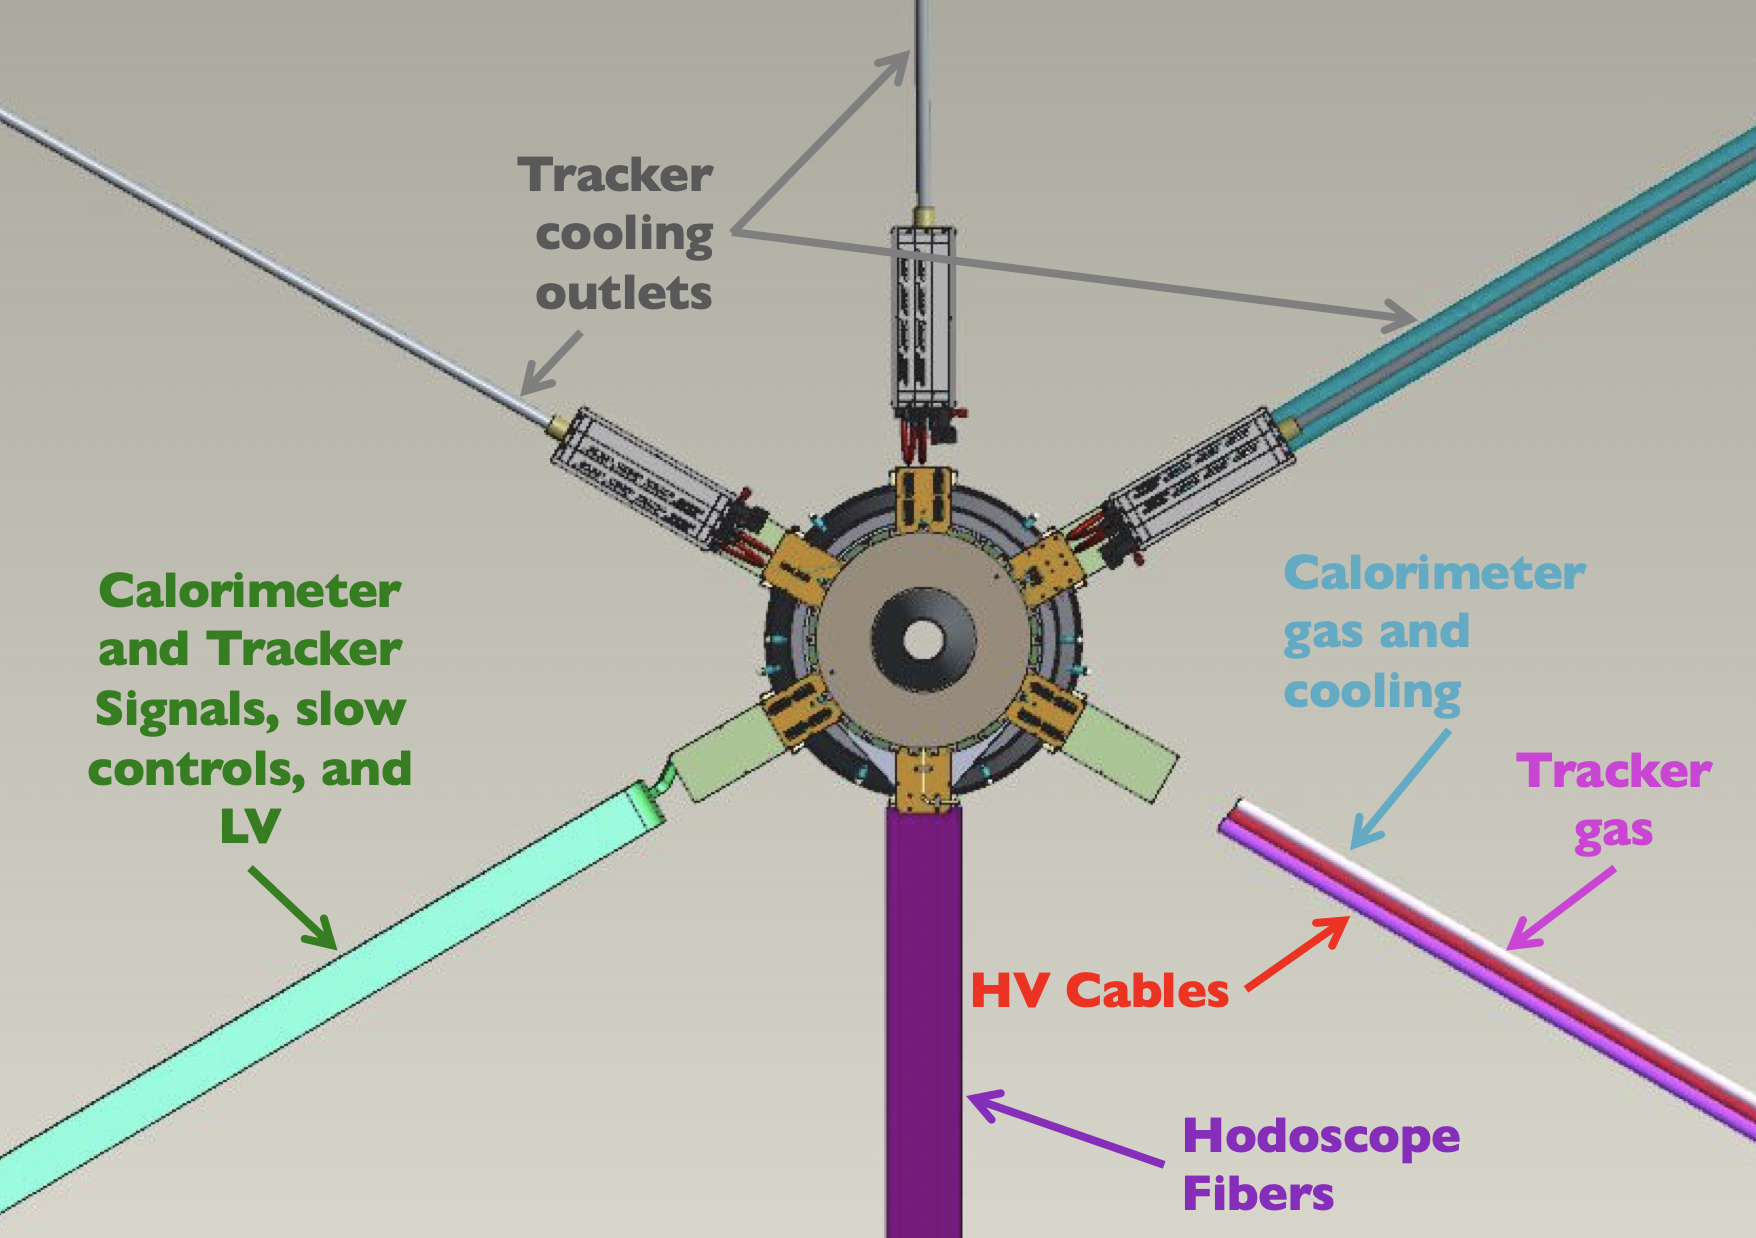
\includegraphics[width=1.0\columnwidth]{./fig/ft_cables.png}
\caption{Front view of the Forward Tagger with the routing of cables and services along the CLAS12 torus coils.}
\label{fig:integra}
\end{figure}

\subsection{Routing of Cabling and Services}

All services and cables necessary for the operation of the FT detectors are routed along the torus coils to minimize
the interference with the CLAS12 Forward Detector as shown in Fig.~\ref{fig:integra}. These include cables for signals
HV, LV, and slow controls, as well as piping for gas distribution and cooling of the three FT subsystems.

The cables and piping are routed along the direction of the magnet coils using appropriate rails. The
width and depth of the rails was chosen to be compatible with the space occupied by the DCs (both during
normal operation and maintenance) and the clearance between the HTCC and the CLAS12 Forward Detector.
